
\documentclass[a4paper,12pt]{article} % добавить leqno в [] для нумерации слева

\usepackage[left=2cm,right=2cm,
top=2cm,bottom=2cm,bindingoffset=0cm]{geometry}

\usepackage[russian, english]{babel} % выбор языка для документа
\usepackage[utf8]{inputenc} % задание utf8 кодировки исходного tex файла
\usepackage[X2,T2A]{fontenc}        % кодировка

\usepackage{fontspec}         % пакет для подгрузки шрифтов
\setmainfont{Times New Roman}       % задаёт основной шрифт документа


 \usepackage{graphicx}
 
\usepackage{amsmath,amsfonts,amssymb,amsthm,mathtools} % AMS
\usepackage{icomma} 
\mathtoolsset{showonlyrefs=true} % Показывать номера только у тех формул, на которые есть \eqref{} в тексте.
%\usepackage{euscript}	 % Шрифт Евклид
%\usepackage{mathrsfs} % Красивый матшрифт
\usepackage{enumitem}
\usepackage{siunitx}
\usepackage{tikz} % To generate the plot from csv
\usepackage{pgfplots}

%%% Заголовок

\newcommand{\latinword}[1]{\textsf{\itshape #1}}%

\begin{document}

{ Касьянова Ксения, СМАР19. Домашняя работа №3. }

\noindent\makebox[\linewidth]{\rule{\textwidth}{0.4pt}}


\section*{Тема 4: цепи Маркова.}
\subsection*{Задача 1}

Пусть

$$Q=\left(\begin{matrix}
\frac{1}{5} & \frac{1}{5} & \frac{3}{5} \\
\frac{1}{5} & 0 & \frac{4}{5} \\
\frac{2}{5} & 0 & \frac{3}{5}
\end{matrix}\right),$$

где $Q$ - переходная матрица ц. м.  $(X_n)$. 

Тогда стационарное распределение $\pi=\left(\pi_{1}, \pi_{2}, \pi_{3}\right)$:

$$\pi Q=\pi, s.t. \sum \pi_i = 1 $$


$$\left(\pi_{1}, \pi_{2}, \pi_{3}\right)\left(\begin{array}{ccc}
\frac{1}{5} & \frac{1}{5} & \frac{3}{5} \\
\frac{1}{5} & 0 & \frac{4}{5} \\
\frac{2}{5} & 0 & \frac{3}{5}
\end{array}\right)=\left(\pi_{1}, \pi_{2}, \pi_{3}\right), s.t. \sum \pi_i = 1 $$


$$\left\{\begin{array}{l}
\frac{1}{5} \pi_{1}+\frac{1}{5} \pi_{2}+\frac{2}{5} \pi_{3}=\pi_{1} \\
\frac{1}{5} \pi_{1}=\pi_{2} \\
\frac{3}{5} \pi_{1}+\frac{4}{5} \pi_{2}+\frac{3}{5} \pi_{3}=\pi_{3}\\
\pi_{1}+\pi_{2}+\pi_{3}=1
\end{array}\right.$$

$$\left\{\begin{array}{l}
\frac{1}{5} \pi_{1}=\pi_{2} \\
\pi_{3}=1 - \frac{6}{5} \pi_{1}\\
\frac{3}{5} \pi_{1}+\frac{4}{5} \cdot \frac{1}{5} \pi_{1}-\frac{2}{5} (1 - \frac{6}{5} \pi_{1} )=0
\end{array}\right.$$

Откуда $\pi_{1} = \dfrac{10}{31}, \pi_{2} = \dfrac{2}{31}, \pi_{3} = 1 - \dfrac{12}{31} =  \dfrac{19}{31}$, т.е. стационарное распределение   \newline
$\pi=\left(\dfrac{10}{31}, \dfrac{2}{31}, \dfrac{19}{31}\right)$.


\subsection*{Задача 2}


Пусть

$$Q=\left(\begin{array}{ccc}
0 & 0 & 1 \\
1 & 0 & 0 \\
0 & \frac{2}{3} & \frac{1}{3}
\end{array}\right)$$

где $Q$ - переходная матрица ц. м.  $(X_n)$. 


Тогда стационарное распределение $\pi=\left(\pi_{1}, \pi_{2}, \pi_{3}\right)$:

$$\pi Q=\pi, s.t. \sum \pi_i = 1 $$


$$\left(\begin{array}{lll}
\pi_{1} & \pi_{2} & \pi_{3}
\end{array}\right)\left(\begin{array}{lll}
0 & 0 & 1 \\
1 & 0 & 0 \\
0 & \frac{2}{3} & \frac{1}{3}
\end{array}\right)=\left(\begin{array}{lll}
\pi_{1} & \pi_{2} & \pi_{3}
\end{array}\right), s.t. \sum \pi_i = 1 $$

$$\left\{\begin{array}{l}
\pi_{2}=\pi_{1} \\
\frac{2}{3} \pi_{3}=\pi_{2} \\
\pi_{1}+\frac{1}{3} \pi_{3}=\pi_{3} \\ \pi_{1}+\pi_{2}+\pi_{3}=1
\end{array}\right. $$

$$\left\{\begin{array}{l}
\pi_{2}=\pi_{1} \\
\frac{2}{3} \pi_{3}=\pi_{2} \\
 \frac{7}{3} \pi_{3} =1
\end{array}\right. $$



Откуда $\pi_{1} = \dfrac{2}{7}, \pi_{2} = \dfrac{2}{7}, \pi_{3} =  \dfrac{3}{7}$, т.е. стационарное распределение   \newline
$\pi=\left(\dfrac{2}{7}, \dfrac{2}{7}, \dfrac{3}{7}\right)$.


\subsection*{Задача 3}


Пусть

$$Q=\left(\begin{array}{lll}
\frac{1}{5} & \frac{1}{5} & \frac{3}{5} \\
\frac{3}{5} & \frac{1}{5} & \frac{1}{5} \\
0 & \frac{3}{5} & \frac{2}{5}
\end{array}\right)$$

где $Q$ - переходная матрица ц. м.  $(X_n)$. 


Тогда стационарное распределение $\pi=\left(\pi_{1}, \pi_{2}, \pi_{3}\right)$:

$$\pi Q=\pi, s.t. \sum \pi_i = 1 $$


$$\left(\begin{array}{lll}
\pi_{1} & \pi_{2} & \pi_{3}
\end{array}\right)\left(\begin{array}{lll}
\frac{1}{5} & \frac{1}{5} & \frac{3}{5} \\
\frac{3}{5} & \frac{1}{5} & \frac{1}{5} \\
0 & \frac{3}{5} & \frac{2}{5}
\end{array}\right) =\left(\begin{array}{lll}
\pi_{1} & \pi_{2} & \pi_{3}
\end{array}\right), s.t. \sum \pi_i = 1 $$

$$\left\{\begin{array}{l}
\frac{1}{5} \pi_{1}+\frac{3}{5} \pi_{2}=\pi_{1} \\
\frac{1}{5} \pi_{1}+\frac{1}{5} \pi_{2}+\frac{3}{5} \pi_{3}=\pi_{2} \\
\frac{3}{5} \pi_{1}+\frac{1}{5} \pi_{2}+\frac{2}{5} \pi_{3}=\pi_{3} \\
\pi_{1}+\pi_{2}+\pi_{3}=1
\end{array}\right.$$

$$\left\{\begin{array}{l}
\pi_{1}=\frac{3}{4} \pi_{2} \\
\pi_{3}= \frac{5}{3} ( \pi_{2}  -  \frac{3}{20} \pi_{2}   - \frac{4}{20} \pi_{2})  =  \frac{13}{12}  \pi_{2}  \\
\frac{3}{4} \pi_{2}+\pi_{2}+ \frac{13}{12}  \pi_{2}=1
\end{array}\right.$$


Откуда $\pi_{1} = \dfrac{9}{34}, \pi_{2} = \dfrac{6}{17}, \pi_{3} =  \dfrac{13}{34}$, т.е. стационарное распределение   \newline
$\pi=\left(\dfrac{9}{34}, \dfrac{6}{17}, \dfrac{13}{34}\right)$.

По эргодической теореме 

$$ 
\lim_{n \to \infty }\frac{1}{n} \sum_{k=0}^{n-1} \mathbb{I}_{\left\{X_{k} \leq 2\right\}} =  \sum_{i\in {\{1,2,3\} } } \mathbb{I}_{\left\{i \leq 2\right\}} \pi(i)  =   \dfrac{9}{34} + \dfrac{6}{17} + 0 =  \dfrac{21}{34}. $$

\subsection*{Задача 4}
  

Пусть

$$Q=\left(\begin{array}{cccc}
\frac{1}{4} & \frac{1}{4} & \frac{1}{3} & \frac{1}{6} \\
\frac{1}{4} & \frac{1}{4} & \frac{1}{4} & \frac{1}{4} \\
0 & \frac{1}{3} & \frac{1}{6} & \frac{1}{2} \\
\frac{1}{2} & \frac{1}{12} & \frac{1}{6} & \frac{1}{4}
\end{array}\right)$$

где $Q$ - переходная матрица ц. м.  $(X_n)$. 


Тогда стационарное распределение $\pi=\left(\pi_{1}, \pi_{2}, \pi_{3}, \pi_{4} \right)$:

$$\pi Q=\pi, s.t. \sum \pi_i = 1 $$


$$\left(\pi_{1} \pi_{2} \pi_{3} \pi_{4}\right)\left(\begin{array}{cccc}
\frac{1}{4} & \frac{1}{4} & \frac{1}{3} & \frac{1}{6} \\
\frac{1}{4} & \frac{1}{4} & \frac{1}{4} & \frac{1}{4} \\
0 & \frac{1}{3} & \frac{1}{6} & \frac{1}{2} \\
\frac{1}{2} & \frac{1}{12} & \frac{1}{6} & \frac{1}{4}
\end{array}\right)=\left(\begin{array}{llll}
\pi_{1} & \pi_{2} & \pi_{3} & \pi_{4}
\end{array}\right), s.t. \sum \pi_i = 1  $$

$$\left\{\begin{array}{ccccc}
-3\pi_{1} &+ \pi_{2}&&+ 2 \pi_{4} &=0 \\
3 \pi_{1} &-9 \pi_{2}&+4 \pi_{3}&+\pi_{4}&=0 \\
4 \pi_{1} &+3 \pi_{2}&-10 \pi_{3}&+2 \pi_{4}&=0 \\
2 \pi_{1} &+3 \pi_{2}&+6 \pi_{3}&-9 \pi_{4}&=0 \\
\pi_{1}&+\pi_{2}&+\pi_{3}&+\pi_{4}&=1
\end{array}\right.$$

Решая методом Гаусса систему уравнений

$$\left(\begin{array}{cccc|c}
-3 & 1 & 0 & 2 & 0 \\
3 & -9 & 4 & 1 & 0 \\
4 & 3 & -10 & 2 & 0 \\
1 & 1 & 1 & 1 & 1
\end{array}\right),$$

получаем стационарное 
распределение   
$\pi=\left(\frac{174}{659}, 
\frac{146}{659},
\frac{151}{659},
\frac{188}{659}
\right)$.

По эргодической теореме 

$$ 
\lim_{n \to \infty } \frac{1}{n} \sum_{k=0}^{n-1}\left(X_{k}\right)^{3}  =  \sum_{i\in {\{1,2,3,4\}} } i^3  \pi(i)  =   1^{3} * \frac{174}{659}+2^{3} * \frac{146}{659}+3^{3} * \frac{151}{659}+4^{3} * \frac{188}{659}=\frac{17451}{659} \approx 26.481$$ 


  
  
\subsection*{Задача 5}
  
  
  
  Пусть
  
$$Q=\left(\begin{array}{ccc}\frac{5}{12} & \frac{1}{3} & \frac{1}{4} \\ \frac{1}{2} & \frac{5}{12} & \frac{1}{12} \\ \frac{5}{12} & \frac{1}{3} & \frac{1}{4}\end{array}\right)$$
  
  где $Q$ - переходная матрица ц. м.  $(X_n)$. 
  
  
  Тогда стационарное распределение $\pi=\left(\pi_{1}, \pi_{2}, \pi_{3}\right)$:
  
  $$\pi Q=\pi, s.t. \sum \pi_i = 1 $$
  
  $$\left(\begin{array}{lll}\pi_{1} & \pi_{2} & \pi_{3}\end{array}\right)\left(\begin{array}{ccc}\frac{5}{12} & \frac{1}{3} & \frac{1}{4} \\ \frac{1}{2} & \frac{5}{12} & \frac{1}{12} \\ \frac{5}{12} & \frac{1}{3} & \frac{1}{4}\end{array}\right)=\left(\begin{array}{lll}\pi_{1} & \pi_{2} & \pi_{3}\end{array}\right), s.t. \sum \pi_i = 1 $$
  
$$\left\{\begin{array}{cccc}
-7 \pi_{1}&+6 \pi_{2}&+5 \pi_{3}&=0\\
4 \pi_{1}&-7 \pi_{2}&+4 \pi_{3}&=0 \\
3 \pi_{1}&+\pi_{2}&-9 \pi_{3}&=0\\
\pi_{1}&+\pi_{2}&+\pi_{3}&=1
\end{array}\right.$$

Решая методом Гаусса систему уравнений


$$\left(\begin{array}{ccc|c}
-7 & 6 & 5 & 0 \\
4 & -7 & 4 & 0 \\
1 & 1 & 1 & 1
\end{array}\right)$$  
получаем стационарное 
распределение   
$\pi=\left(\frac{59}{132}, 
\frac{4}{11},
\frac{25}{132}
\right)$.

По эргодической теореме 

$$ 
\lim_{n \to \infty }\frac{1}{n} \sum_{k=0}^{n-1} \mathbb{I}_{\left\{X_{k} = 1 \right\}} =  \sum_{i\in {\{1,2,3\} } } \mathbb{I}_{\left\{i = 1 \right\}} \pi(i)  =   \dfrac{59}{132} + 0 + 0 =  \dfrac{59}{132}. $$

  
\subsection*{Задача 6}

Пусть начальное распределение ц. м. 
$\mu^{(0)}=\left(\frac{2}{7}, \frac{5}{7}\right)$, а матрица перехода: 

$$P=\left(\begin{array}{ll}
1 / 3 & 2 / 3 \\
2 / 5 & 3 / 5
\end{array}\right)$$. 

Тогда функцию инициирования $\psi(x)$ для $\mu^{(0)}$  можно задать как 

$$\psi(x)=\left\{\begin{array}{ll}
1, & x \in\left[0, \frac{2}{7}\right) \\
2, & x \in\left[\frac{2}{7}, 1\right]
\end{array}\right.. $$

Пусть $U_{0}, U_{1}, \ldots \sim  U[0,1] \ i.i.d.$. 
Тогда  $X_{0}=\psi\left(U_{0}\right) \sim \mu^{(0)}$ задает начальное распределение. 

Функция обновления строится аналогично (но роль  $\mu^{(0)}$ i-ая строка переходной матрицы): 

$$\phi(1, x)=\left\{\begin{array}{ll}
1, & x \in\left[0, \frac{1}{3}\right) \\
2, & x \in\left[\frac{1}{3}, 1\right]
\end{array}\right.$$
 

$$\phi(2, x)=\left\{\begin{array}{ll}
1, & x \in\left[0, \frac{2}{5}\right) \\
2, & x \in\left[\frac{2}{5}, 1\right]
\end{array}\right.$$


Далее итеративно моделируется цепь маркова с заданным начальным распределением и  матрицей перехода:

  $$X_{0}=\psi\left(U_{0}\right), X_{1}=\phi\left(X_{0}, U_{1}\right), X_{2}=\phi\left(X_{1}, U_{2}\right),  \dots, X_{k}=\phi\left(X_{k-1}, U_{k}\right)$$




\subsection*{Задача 7}



Пусть начальное распределение ц. м. 
$\mu^{(0)}=\left(\frac{2}{7}, \frac{1}{7}, \frac{4}{7}\right)$, а матрица перехода: 

$$P=\left(\begin{array}{ccc}
1 / 2 & 1 / 4 & 1 / 4 \\
1 & 0 & 0 \\
1 / 3 & 1 / 3 & 1 / 3
\end{array}\right)$$

Тогда функцию инициирования $\psi(x)$ для $\mu^{(0)}$  можно задать как 

$$\psi(x)=\left\{\begin{array}{ll}
1, & x \in\left[0, \frac{2}{7}\right) \\
2, & x \in\left[\frac{2}{7}, \frac{3}{7}\right) \\
3, & x \in\left[\frac{3}{7}, 1\right]
\end{array}\right.$$

Пусть $U_{0}, U_{1}, \ldots \sim  U[0,1] \ i.i.d.$. 
Тогда  $X_{0}=\psi\left(U_{0}\right) \sim \mu^{(0)}$ задает начальное распределение. 

Функция обновления строится аналогично (но роль  $\mu^{(0)}$ i-ая строка переходной матрицы): 

$$\phi(1, x)=\left\{\begin{array}{ll}
1, & x \in\left[0, \frac{1}{2}\right) \\
2, & x \in\left[\frac{1}{2}, \frac{3}{4}\right) \\
3, & x \in\left[\frac{3}{4}, 1\right]
\end{array}\right.$$

$$\phi(2, x)= 1, \  x \in[0,1]  $$

$$\phi(3, x)=\left\{\begin{array}{ll}
1, & x \in\left[0, \frac{1}{3}\right) \\
2, & x \in\left[\frac{1}{3}, \frac{2}{3}\right) \\
3, & x \in\left[\frac{2}{3}, 1\right]
\end{array}\right.$$

Далее итеративно моделируется цепь маркова с заданным начальным распределением и  матрицей перехода:

$$X_{0}=\psi\left(U_{0}\right), X_{1}=\phi\left(X_{0}, U_{1}\right), X_{2}=\phi\left(X_{1}, U_{2}\right),  \dots, X_{k}=\phi\left(X_{k-1}, U_{k}\right)$$




\subsection*{Задача 8}

Пусть стационарное распределение ц. м., заданной на графе $\pi=\left(\frac{2}{9}, \frac{4}{9}, \frac{1}{3}\right)$, и известно, что $d_{1}=d_{2}=d_{3}=2$.

Тогда переходная матрица цепи Маркова находится следующим образом: 

$$\begin{aligned}
P_{12}=& \frac{1}{d_{1}}\left(\frac{\pi_{2}}{\pi_{1}} \cdot \frac{d_{1}}{d_{2}} \wedge  1\right)=\frac{1}{2}\left(2\wedge 1\right)=\frac{1}{2} \\
P_{13}=& \frac{1}{d_{1}}\left(\frac{\pi_{3}}{\pi_{1}} \cdot \frac{d_{1}}{d_{3}} \wedge 1\right)=\frac{1}{2}\left(\frac{3}{2}\wedge 1\right)=\frac{1}{2} \\ P_{11}=& 1-\frac{1}{2}-\frac{1}{2}=0
\end{aligned}$$


$$\begin{aligned}
P_{21}=& \frac{1}{d_{2}}\left(\frac{\pi_{1}}{\pi_{2}} \cdot \frac{d_{2}}{d_{1}} \wedge {1}\right)=\frac{1}{2}\left(\frac{1}{2} \wedge {1}\right)=\frac{1}{4} \\
P_{23}=& \frac{1}{d_{2}}\left(\frac{\pi_{3}}{\pi_{2}} \cdot \frac{d_{2}}{d_{3}} \wedge 1 \right)=\frac{1}{2}\left(\frac{3}{4} \wedge 1\right)=\frac{3}{8} \\
 P_{22}=&1-\frac{1}{4}-\frac{3}{8}=\frac{3}{8}
\end{aligned}$$


$$\begin{aligned}
P_{31}=& \frac{1}{d_{3}}\left(\frac{\pi_{1}}{\pi_{3}} \cdot \frac{d_{3}}{d_{1}}\wedge1\right)=\frac{1}{2}\left(\frac{2}{3}\wedge 1\right)=\frac{1}{3} \\
P_{32}=& \frac{1}{d_{3}}\left(\frac{\pi_{2}}{\pi_{3}} \cdot \frac{d_{3}}{d_{2}}\wedge1\right)=\frac{1}{2}\left(\frac{4}{3}\wedge 1\right)=\frac{1}{2} \\
  P_{33}&=1-\frac{1}{2}-\frac{1}{3}=\frac{1}{6}
\end{aligned}$$



$$P=\left(\begin{array}{ccc}
0 & \frac{1}{2} & \frac{1}{2} \\
\frac{1}{4} & \frac{3}{8} & \frac{3}{3} \\
\frac{1}{3} & \frac{1}{2} & \frac{1}{6}
\end{array}\right)$$

\newpage 

Граф с вероятностями перехода


% TODO: \usepackage{graphicx} required
\begin{figure}[h!]
	\centering
	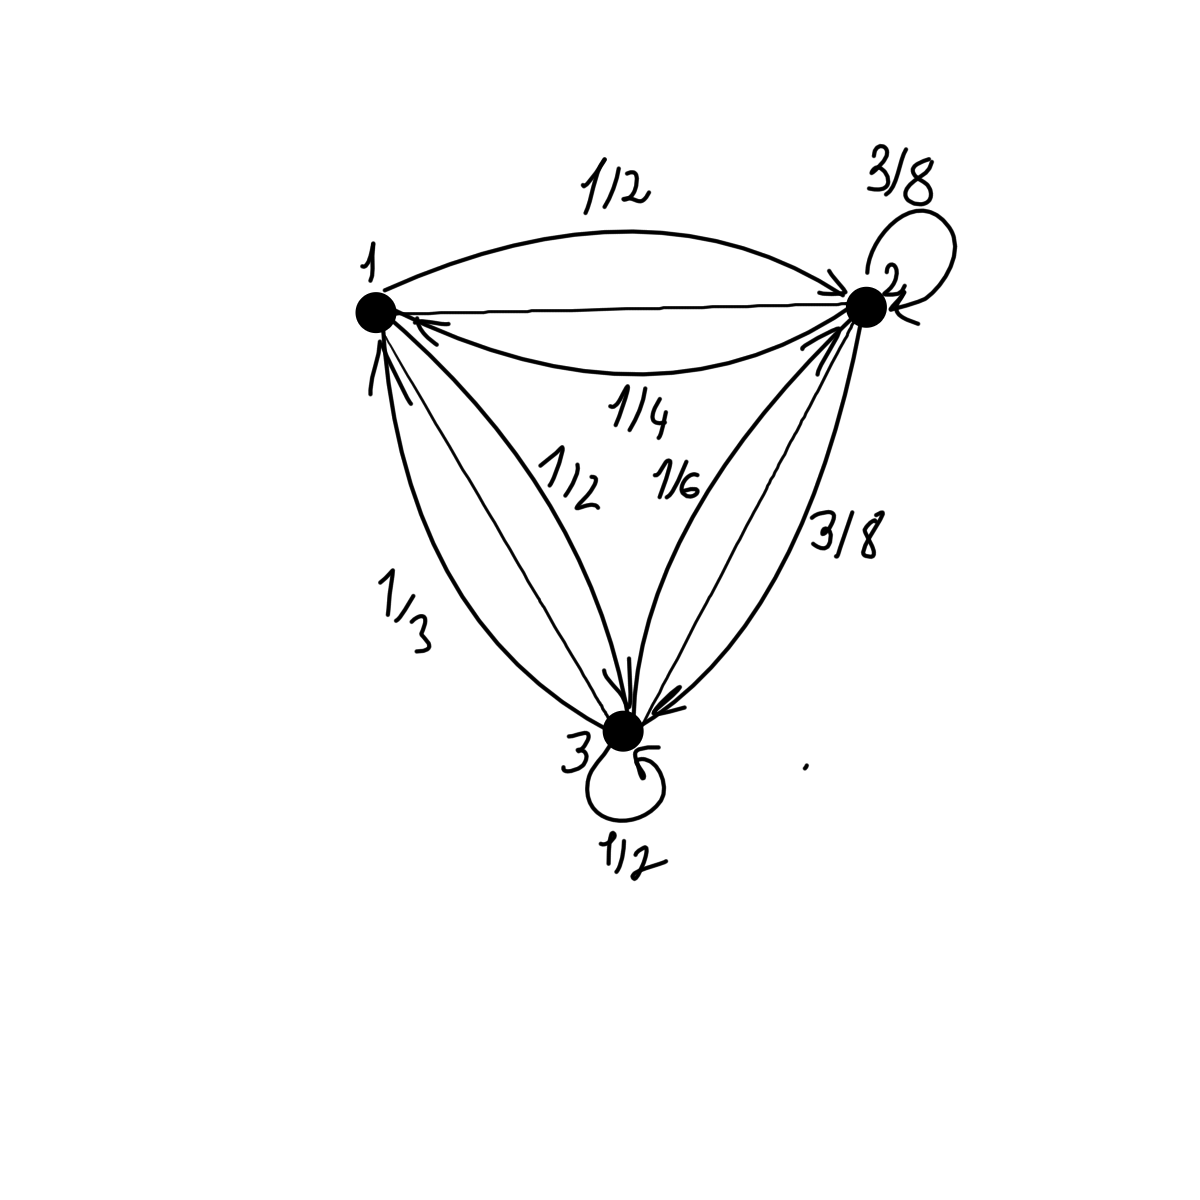
\includegraphics[width=0.7\linewidth]{screenshot001}
	\label{fig:screenshot001}
\end{figure}


Полученное распределение является стационарным, поскольку с помощью подстановки легко видеть, что выполняется  

$$\left(\begin{array}{lll}
\pi_{1} & \pi_{2} & \pi_{3}
\end{array}\right)\left(\begin{array}{lll}
0 & \frac{1}{2} & \frac{1}{2} \\
\frac{1}{4} & \frac{3}{8} & \frac{3}{3} \\
\frac{1}{3} & \frac{1}{2} & \frac{1}{6}
\end{array}\right)  = \left(\begin{array}{lll}
\pi_{1} & \pi_{2} & \pi_{3}
\end{array}\right) $$

при  $$\pi_{1}+\pi_{2}+\pi_{3}=1 $$  




\subsection*{Задача 9}


Пусть стационарное распределение ц. м., заданной на графе $\pi=\left(\frac{1}{3}, \frac{1}{3}, \frac{1}{3}\right)$, и известно, что $d_{1}=2, d_{2}=d_{3}=1$.

Тогда переходная матрица цепи Маркова находится следующим образом: 



$$\begin{aligned}
P_{12}=\frac{1}{d_{1}}\left(\frac{\pi_{2}}{\pi_{1}} \cdot \frac{d_{1}}{d_{2}} \wedge 1\right) &=\frac{1}{2}\left(1 * 2  \wedge 1\right)=\frac{1}{2} \\
P_{13}=\frac{1}{d_{1}}\left(\frac{\pi_{3}}{\pi_{1}} \cdot \frac{d_{1}}{d_{3}}  \wedge 1\right) &=\frac{1}{2}\left(1 * 2\wedge 1\right)=\frac{1}{2} \\ P_{11}& =1-\frac{1}{2}-\frac{1}{2}=0
\end{aligned}$$


$$\begin{array}{c}
P_{23}=0 \\
P_{21}=\frac{1}{d_{2}}\left(\frac{\pi_{1}}{\pi_{2}} \cdot \frac{d_{2}}{d_{1}}\wedge 1\right)=\left(\frac{1}{2}\wedge 1\right)=\frac{1}{2} \\
P_{22}=1-\frac{1}{2}=\frac{1}{2}
\end{array}$$



$$\begin{array}{c}
P_{32}=0 \\
P_{31}=\frac{1}{d_{3}}\left(\frac{\pi_{1}}{\pi_{3}} \cdot \frac{d_{3}}{d_{1}}\wedge1\right)=\left(\frac{1}{2}\wedge 1\right)=\frac{1}{2} \\
 P_{33}=1-\frac{1}{2}=\frac{1}{2}
\end{array}$$


$$P=\left(\begin{array}{ccc}
0 & \frac{1}{2} & \frac{1}{2} \\
\frac{1}{2} & \frac{1}{2} & 0 \\
\frac{1}{2} & 0 & \frac{1}{2}
\end{array}\right)$$


Граф с вероятностями перехода


% TODO: \usepackage{graphicx} required
\begin{figure}[h!]
	\centering
	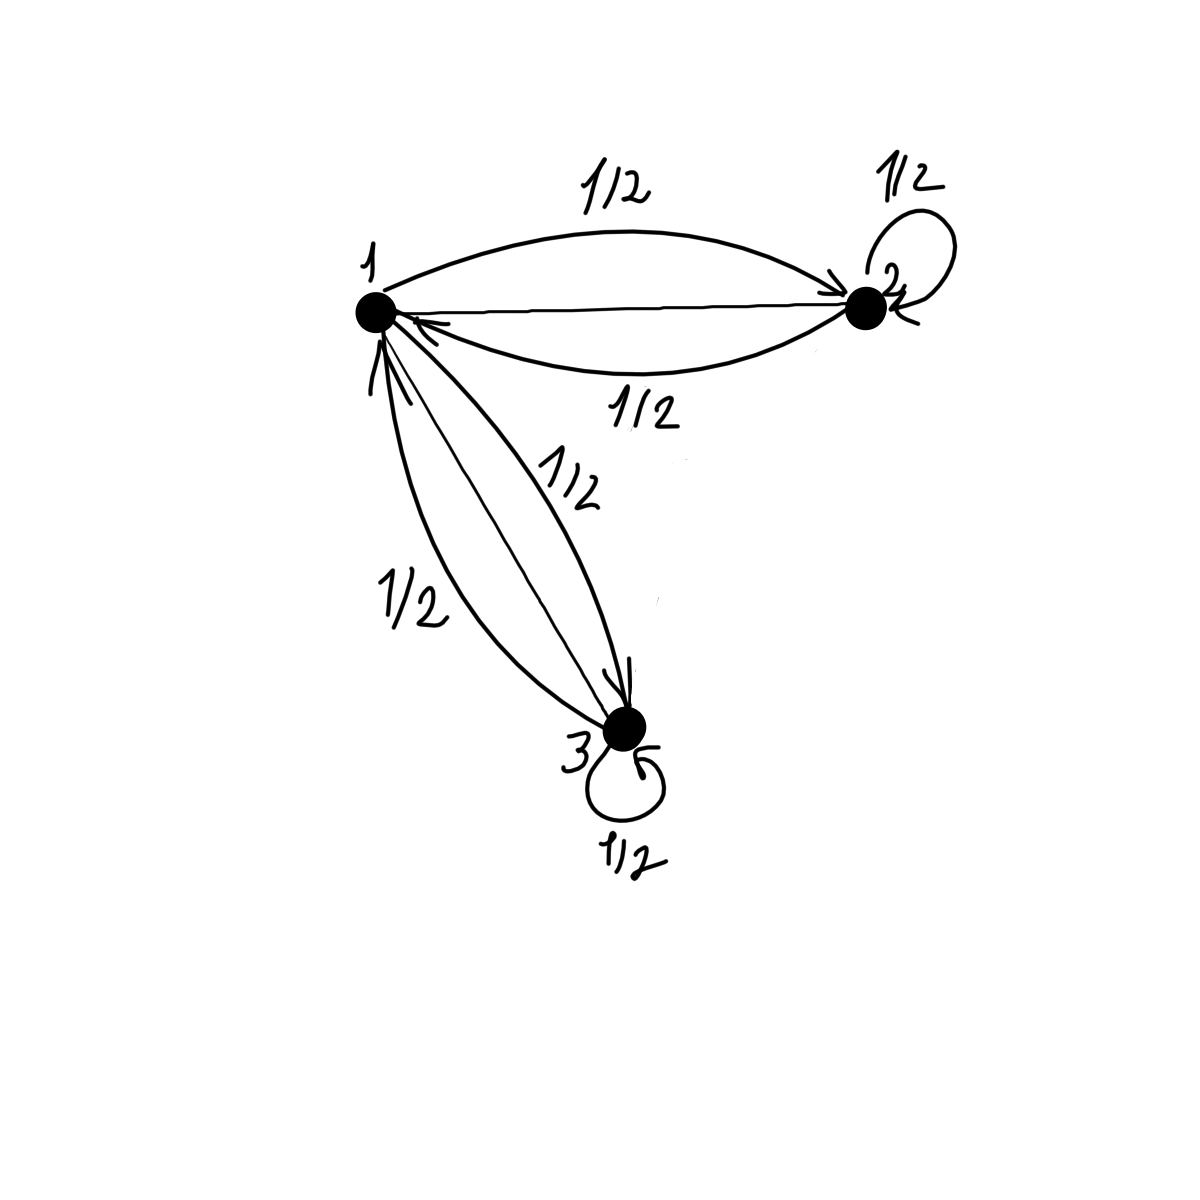
\includegraphics[width=0.7\linewidth]{screenshot002}
	\label{fig:screenshot001}
\end{figure}




Полученное распределение является стационарным, поскольку с помощью подстановки легко видеть, что выполняется  

$$\left(\begin{array}{lll}
\pi_{1} & \pi_{2} & \pi_{3}
\end{array}\right)\left(\begin{array}{lll}
0 & \frac{1}{2} & \frac{1}{2} \\
\frac{1}{2} & \frac{1}{2} & 0 \\
\frac{1}{2} & 0 & \frac{1}{2}
\end{array}\right) =\left(\begin{array}{lll}
\pi_{1} & \pi_{2} & \pi_{3}
\end{array}\right)  $$

при  $$\pi_{1}+\pi_{2}+\pi_{3}=1 $$  


\end{document}